\documentclass[fontsize=11pt]{article}  
  
\usepackage{amsmath}  
  
\usepackage[utf8]{inputenc}  
\usepackage{graphicx}
  
\usepackage[margin=0.75in]{geometry}  
\title{CSC110 Project Report: Predicting COVID-19 Infection Fatality Rate Based On Percentage Of Population Vaccinated Using Regression Modelling}  
  
\author{Sunghyoun Kim, Arsal Khan, Maroosh Gillani, John Fitzgerald}  
  
\date{Tuesday, December 14, 2021}  
  
  
\begin{document}  
  
\maketitle  
  
  
\section*{Problem Description and Research Question}  
  
  
\textbf{Is there a relationship between the percentage of a population vaccinated and the Infection Fatality Rate of COVID-19?}  
  
  
Considering its impact on everyone’s lives for the past two years, the majority of the human population is familiar with the rise of COVID-19 at the start of 2020. What was supposed to be a two-week lockdown turned into a nearly two-year roller-coaster of lockdowns and restrictions.  
  
  
The start of 2021 however, was a ray of hope for many people as vaccine doses were being administered to members of the public. The rollout of vaccines persuaded many into believing that the whole COVID-19 ordeal may be over soon. However, this came with many conspiracy theorists claiming the vaccine was a hoax and began questioning its safety for human use (Islam at al., 2021). The following months became a battle between public health experts and the lay anti-vaxxer, the former trying to prove the safety of vaccine use, and the latter looking for any excuse to dismiss the appropriate use of the vaccine (PublicHealth.org, 2021). Several government institutions in Canada implemented campaigns to increase the percentage of the population vaccinated, such as proposing vaccine lotteries with receiving a dose of the vaccine as an entry ticket (Rastello, 2021). Other governments took a different approach with vaccine mandates and restricting non-essential public services to those who have proof of vaccination (Kirschbaum, 2021).   
  
The controversy on vaccine effectiveness is what motivates our research question. Our goal is to research the correlation or lack thereof between the percentage of the population vaccinated(Fully) or \textbf{\%PV}, versus the COVID-19 Infection Fatality Rate or \textbf{``IFR"}, which is the percentage of confirmed deaths per Infected Case. Since it was not possible to accurately measure every occuring case, we used the reproduction rate of COVID-19 in a given area as a substitute. Our goal then is to generate a regression model which predicts the IFR based on the \%PV. Another point of interest would be how effective the vaccine seems to be in various nations. Whether it be the speed of the rollout or the type of vaccine used, how have vaccines affected COVID-19 Infection Fatality Rates?   
  
  
\section*{Dataset Description}  

The dataset to be used is a modified version of the original dataset ‘Our World in Data, COVID-19’. Its source is the website ourworldindata.org, a project of the non-profit organization Global Change Data Lab. The type of the dataset is in csv. The modified version only contains the data of the countries Canada, United States, United Kingdom, France, Germany, and Australia in particular, as these countries have the most consistent data available. It covers a variety of COVID-19 related metrics for various countries. 

In particular, this project analyzes and compares the metrics: 'location', 'new\_deaths\_smoothed\_per\_million', 'people\_fully\_vaccinated\_per\_hundred', and 'reproduction\_rate'.
  
We will be using 7-day rolling averages for our new cases and new deaths values.   
This is expressed by the ``smoothed" suffix.   
This is to account for minor deviances per day and eliminate day-to-day outliers.  
\newpage  
  
  
  
\section*{Computational Plan}  
  
  
Our computational overview revolves around training a machine learning model to accurately predict how the IFR(Infection Fatality Rate) is affected by the \%PV(Percent of Population Fully Vaccinated). We went about this by:  
  
  
\begin{enumerate}
    \item Processing Raw data from CSV. In this step, we filter the data to only contain the countries and columns we require. Namely, location, vaccinated\_per\_hundred, new\_deaths\_smoothed, and reproduction\_rate. We create a Country class to store this data and store the indivdual values as numpy arrays belonging to the class. We include a function to compute the IFR from the new\_deaths\_smoothed and reproduction\_rate values.  
    For this step, we will be using the python library NumPy and the built-in library: csv. All operations are done within data\_filtering.py.
      
    \item Fitting to the regression model. With this data, we now fit it into a linear regression model which will allow us to make predictions for future \%PV values. We first define the base function
        \[
            2^{ax + b}
        \]
        
        
    Through a series of iterations, we found this to adjust best to the varying IFR data of different countries. We believe this is due the exponential nature of a pandemic's spread. 


    After creating a Model class to store our data and functions, we assign x and y values to use for our model training using scikit-learn's train\_test\_split() function. We then use the scipy optimize.curve.fit() function to train our model and obtain our a and b coefficients.

    Now that we have our a and b values, we run the function on the domain 0-100 to see the outputs of all possible \%PVs.


    We also defined a test function get\_ifr() to output the IFR at any given percentage.
    For this step, we take advantage of NumPy arrays and then feed them into our scikit-learn and scipy functions to define and fit our data to the model.   

    
    All operations are done within data\_computations.py.
      
\item Data visualization. After we train our model, we use Matplotlib to generate visualizations with our data that show how well our regression model fits the line to our data. The visualizations are a scatter plot with the inclusion of our regression line. With \%PV on the x-axis and our IFR on the y-axis. It is plotted onto an interactive window that allows you to toggle the different lines and compare the different countries' IFR and \%PV correlation. A legend is included. This visualization allows us to test our original hypothesis and reach a conclusion to our research question. For this, a Plot class is created to take in a list of different country Models and to take in a list of possible colors, as matplotlib color codes.

    For this step, we take advantage of Matplotlib's Pyplot and Widgets sub-libraries along with NumPy arrays. 

    All operations are done within data\_visualizaion.py.
  
\end{enumerate}  
  
A new library we will be using is SciPy and Scikit-learn. Both used for machine learning, it provides efficient and simple tools for predictive data analysis which will be useful since we will be using a regression model to predict the future IFR. In regards to regression modelling, SciPy provides a variety of tools which facilitate the process of training/fitting our model, namely optimize.fit\_curve, which we will be using in our data\_computations file. Scikit-learn is built on NumPy and SciPy, while being Open source, and commercially usable from the BSD license, meaning it is available to use for our project.  
  
  

\section*{Instructions for Obtaining Data Sets and Running the Program}

Please install all Python libraries listed under the `requirements.txt' file, which can be obtained from MarkUs.

As mentioned in the Dataset description, we use a modified version of the original dataset ‘Our World in Data, COVID-19’. As such, the it is submitted to MarkUs and is available to be directly downloaded from there. Please save this dataset in the same directory as the python files.


After running main.py, the TA should expect to see an interactive window popup containing a set of checkboxes, a plot, and a legend.
If the TA is running pycharm, the window will open as an image within the tool window as an image rather than an app.
In this case, they should go to File | Settings | Tools | Python Scientific and toggle "Show plots in tool window" to open the app outside of pycharm.
They will also be able to manipulate the main.py file and try out different countries.

\begin{figure}[htbp]
    \centerline{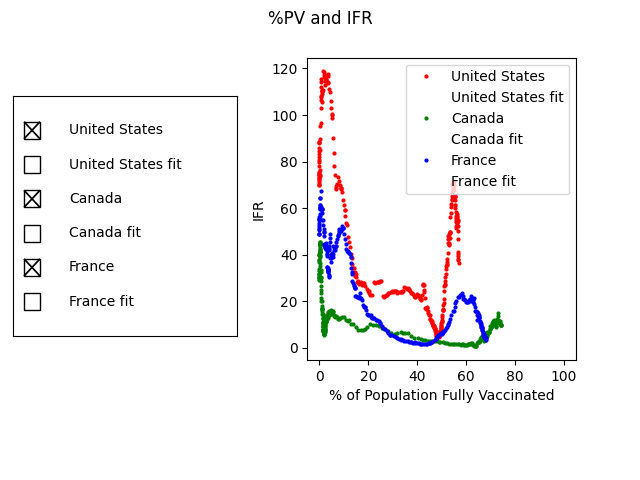
\includegraphics{Figure_1.png}}
    \caption{The checkboxes on the left are clicked to toggle the visibility of the graphs. (See Figure 2)}
\label{fig}
\end{figure}

\begin{figure}[htbp]
\centerline{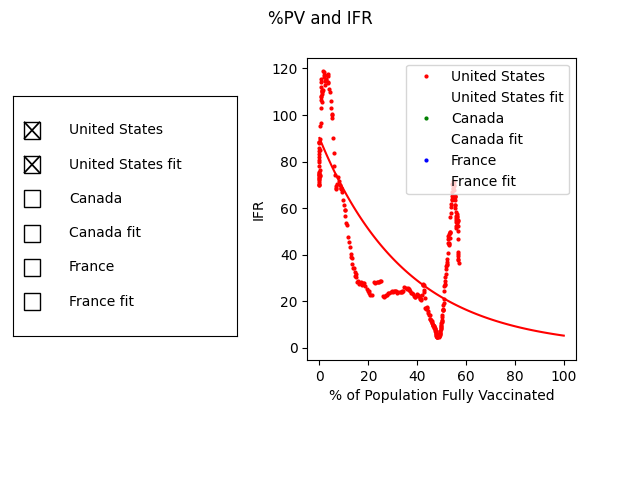
\includegraphics{Figure_2.png}}
\label{fig}
\end{figure}
\section*{Changes from Proposal}


We changed our dependant variable from CFR to IFR due to an eye-opening realization of the failures of CFR as an accurate metric to predict the true lethality of a disease. See source [10]. \\
We also changed the training function to SciPy's curve\_fit() rather than Scikit-learn's LinearRegression class as it was better adapted to our base mathematical model.Hannah Ritchie, Edouard Mathieu, Lucas Rodés-Guirao, Cameron Appel, Charlie Giattino, Esteban Ortiz-Ospina, Joe Hasell, Bobbie Macdonald, Diana Beltekian and Max Roser (2020) - "Coronavirus Pandemic (COVID-19)". Published online at OurWorldInData.org. Retrieved from: 'https://ourworldindata.org/coronavirus' [Online Resource]
Moreover, we decided against using the pandas library and instead adapted our code into an object based programming approach, in order to improve readability and code structure. Furthermore, we decided to incorporate an interactive element to the plots which allow users to toggle between the graphs of different countries in order to make our visuals more interesting and to simultaneously add complexity in an interesting manner.


\section*{Discussion}


%From the handout --> Do the results of your computational exploration help answer this question?
% What limitations did you encounter, with the datasets you found, the algorithms/libraries you used, or other obstacles?
% What are some next steps for further exploration?

Through this project, we learned that the answer to our question is that as more vaccinations are becoming increasingly available to the public, the amount of people dying due to COVID-19 is indeed generally decreasing. By utilizing linear regression, we were able to obtain a graph that shows the general trend of IFR per \%PV up to a certain percentage of \%PV. For example, in Canada, the vaccinated population percentage was 70\% as per our dataset, and we were able to predict the IFR at 100\% \%PV. This was done by looking at the extended graph obtained from our code, which revealed that regardless of the vaccine's effect on case count, it is succeeding in reducing the number of deaths. This will continue to happen as found from our predictor since the \%PV of our population will only increase with time. 


Some next steps for further exploration are to complete a linear regression analysis for less-developed countries around the world since our project was using developed countries COVID-19 data. This will allow us to compare and contrast between the differences in our predictions for IFR in developed and less-developed countries. 

Another way we can further explore our topic is to conduct the same project using a non-linear regression analysis. By doing this, we can compare directly with our already completed linear regression predictor how the IFR values differ based on different \%PV values.






\section*{References}  
  
\begin{enumerate}  
    \item Harrington, R. A. (n.d.). Case fatality rate. Encyclopædia Britannica. Retrieved December 13, 2021, from https://www.britannica.com/science/case-fatality-rate.   
    \item Harris, C. R., Millman, K. J., van der Walt, S. J., Gommers, R., Virtanen, P., Cournapeau, D., Wieser, E., Taylor, J., Berg, S., Smith, N. J., Kern, R., Picus, M., Hoyer, S., van Kerkwijk, M. H., Brett, M., Haldane, A., del Río, J. F., Wiebe, M., Peterson, P., … Oliphant, T. E. (2020, September 16). Array programming with NumPy. Nature. Retrieved December 13, 2021, from https://doi.org/10.1038/s41586-020-2649-2. 
    \item Pedregosa, F., Varoquaux, G., Gramfort, A.,  Michel, V., Thirion, B., Grisel, O., Blondel, M., Prettenhofer, P., Weiss, R., Dubourg, V., Vanderplas, J., Passos, A. \& Cournapeau, D., (2011). Journal of Machine Learning Research 12. pp. 2825–2830. Retrieved December 13, 2021.
    \item Ritchie, H., Mathieu, E., Rodés-Guirao, L., Appel, C., Giattino, C., Ortiz-Ospina, E., Hasell, J., Macdonald, B., Beltekian, D., \& Roser, M. (2020, March 5). Coronavirus pandemic (COVID-19) - statistics and Research. Our World in Data. Retrieved December 13, 2021, from https://ourworldindata.org/coronavirus. 
    \item Islam, M. S., Kamal, A. H. M., Kabir, A., Southern, D. L., Khan, S. H., Hasan, S. M., ... \& Seale, H. (2021). COVID-19 vaccine rumors and conspiracy theories: The need for cognitive inoculation against misinformation to improve vaccine adherence. PloS one, 16(5), e0251605.
    \item Kirschbaum, E. (2021, November 18). Germany bans unvaccinated from public transport and warns of 'bleak' Christmas. The Independent. Retrieved December 13, 2021, from https://www.independent.co.uk/news/world/europe/germany-covid-vaccinations-christmas-transport-b1960065.html. 
    \item PublicHealth.org. (2021, October 14). Vaccine myths debunked. PublicHealth.org. Retrieved December 13, 2021, from https://www.publichealth.org/public-awareness/understanding-vaccines/vaccine-myths-debunked/. 
    \item Rastello, S. (2021, June 16). Canada’s Virus Hot Zone Adopts Lottery to Boost Vaccinations. Bloomberg.com. Retrieved December 13, 2021, from https://www.bloomberg.com/news/articles/2021-07-16/canada-s-virus-hot-zone-adopts-lottery-to-boost-vaccinations. 
    \item McKinney, W. (n.d.). Data Structures for Statistical Computing in Python. conference.scipy. Retrieved December 13, 2021, from http://conference.scipy.org/proceedings/scipy2010/pdfs/mckinney.pdf. 
    \item Hannah Ritchie, Edouard Mathieu, Lucas Rodés-Guirao, Cameron Appel, Charlie Giattino, Esteban Ortiz-Ospina, Joe Hasell, Bobbie Macdonald, Diana Beltekian and Max Roser (2020) - "Coronavirus Pandemic (COVID-19)". Published online at OurWorldInData.org. Retrieved from: 'https://ourworldindata.org/coronavirus' [Online Resource] 
\end{enumerate}  
% NOTE: LaTeX does have a built-in way of generating references automatically,  
  
% but it's a bit tricky to use so we STRONGLY recommend writing your references  
  
% manually, using a standard academic format like APA or MLA.  
  
% (E.g., https://owl.purdue.edu/owl/research_and_citation/apa_style/apa_formatting_and_style_guide/general_format.html)  
  
  
\end{document}
